%!TEX root = thesis.tex
\chapter{Technical Specification} % (fold)
\label{ch:implementation}
This section describes a technical specification of a direct implementation of the design choices made in the previous chapter in terms of client side and server side tasks.

The proposed design presented in the previous chapter has accounted for the presented requirements and user needs, but there are some requirements that will not be implemented due to prioritisation and time limits.

The in chapter~\ref{ch:design} presented application incorporates the user model, but this chapter will only present how to collect the necessary user data and use it in the application -- and not implement it. It will, however, describe which meta data is needed and how to acquire it.

The social aspects of the system is of cause an important part of it and in terms of the business case, social media are easy channels for awareness. \cite{Tidwell} even states her editorial mix pattern as a social media pattern. Nonetheless, these will not be implemented in the presented application as it does not contribute with new knowledge to field. The gathered news articles to used in this project contained both images and videos, but only images will be considered here. It is however easy to implement the support for videos as the same space allocation principles applies.

Also, the personalised summaries have already been very well explored in the paper \cite{fulltext.pdf} and this project will not try to compete with it, so only the first few sentences will constitute the excerpts from articles to be used on the front page.

The categories used to compose sections of is by no means a full list and they have not been verified, but they are some of the most recurring in popular news sites and are used just in order to proof the concept is possible. Thus, their definitions are not comprehensive either.

Finally, only a selection of the full list of the editorial mix constraints, presented in the proposed design, will be implemented. Furthermore, before the user test was done the implementation had already started leading to the implementation of a fairly complex layout constraint to minimise white space. It turned out that some white space was actually a user preference, but the implementation of the constraint will be presented nonetheless, as it shows a good example of what is possible with the system. 
%
%Whitespace between articles should be minimised. This is not an actual user requirement, but it is included as it a fairly complex layout problem to solve and it shows some aspects of what it can do.


\section{Server for Acquiring and Mining Data for Personalisation}
%\subsection{Spacial, temporal and relational personalisation}
The \cite{DCMI} proposes 15 meta data elements for documents, i.e.\ Title, Creator, Subject, Description, Publisher, Contributor, Date, Type, Format, Identifier, Source, Language, Relation, Coverage and Rights. The articles in this project have been acquired using the \cite{Readability} to scrape web pages of articles given by links from RSS-feeds. This way it is possible to get the full article. Under normal circumstances, these would probably be supplied by a content provider, say through an agreement with newspaper companies or social networks. The Readability API provides several meta data elements for the parsed articles; a domain, a title, a article URL, a URL for a lead image, the author, an article excerpt, a word count and a date of publish. This satisfies many of our needs, but there are still some very crucial calculations to be done, i.e.\ the article relevance according to user topics and similarity between articles.

The analysis of article relevance and similarity to other articles will use the same two types analysis, namely a document using the WordNet and entity comparison using Open Calais. These will be presented in the following two sections.

\todo[inline]{Er der argumenteret for at bruge keywords?}

\subsection{WordNet Enriching Articles}
WordNet is a large lexical database of English words and their relationships in the form of different graphs. WordNet is based on \emph{synsets}, which is a set of synonyms which describes different meanings of the same word. WordNet has hyperonymy and hyponymy graph for noun synsets, which is based on the ISA relation between words. A \emph{hypernym} relation is a generalisation, e.g.\ a hypernym for a bed is a piece of furniture; and a \emph{hyponym} relation is a specification, e.g.\ a hyponym for a bed is a bunkbed. For nouns there also exists the meronymy graph, which is a graph describing the part-whole relation; a chair e.g.\ has a back, a seat and legs. Also, parts are inherited by superordinates, e.g.\ if a chair has legs, then an armchair has legs as well. Furthermore, WordNet has a graph describing elaboration, i.e.\ \emph{troponyms}, of verbs synsets, adjectives organised in terms of antonymy and adverbs which can be be described in terms of adjectives. The synsets, the hypernym and hyponym graph and the troponym graph of WordNet are the most interesting, because they describe different meaning of a given word, whereas the others describes relation to other words.
%Noun hyperonymy, hyponymy or ISA relation
%Noun Meronymy, inherited
%Verb synsets, troponyms: dimensions along which verbs can be elaborated
%Adjectives are organized in terms of antonymy
%adverbs are straightforwardly derived from adjectives via morphological affixation

The initial approach involved computing the tf-idf similarity between articles and the topics and articles in between using the Python libraries for this \cite{NLTK}. This approach works on a bow (bag-of-words) with key words and weights representing a single item. The weight is computed by the number of occurrences in the provided text and a cosine distance determines the similarity. However, Python also provides an interface for working with WordNet. This opens the door to a more in-depth analysis of the obtained news articles. \cite{116262780379.pdf} presents an algorithm for enriching articles using WordNet's hypernym graph. A subgraph of WordNets hypernym graph is generated by the top $20\%$ frequent keywords of an article and weighted by:
$$W(d, f) = 2 \cdot \frac{1}{1+e^{-0.125(d^3\frac{f}{TW})}}-0.5$$

Where $d$ stands for the node's depth in the graph (starting from root and moving downwards), $f$ is the frequency of appearance of the node to the multiple graph paths and $TW$ is the total number of words used to generate the hypernym graph. An example of such a hypernym graph is seen in Figure~\ref{fig:hypernym-graph}.
\begin{figure}[h!tp]
	\myfloatalign
	%\makebox[\textwidth][l]{
		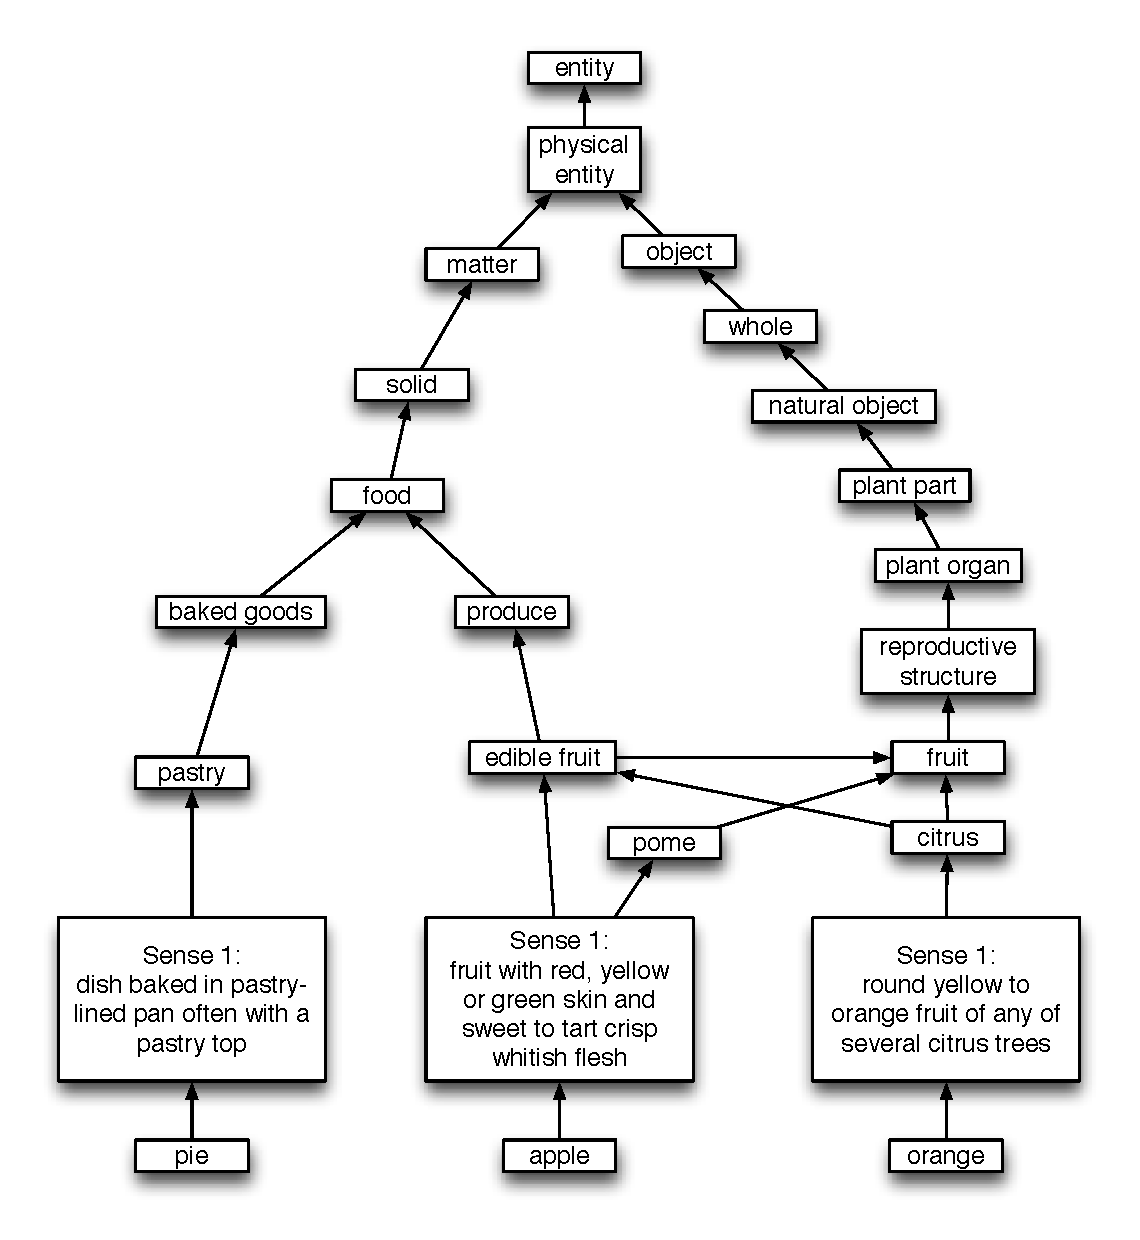
\includegraphics[width=.8\textwidth]{img/hypernym-graph}
	%}
	%\marginnote{
		%\begin{minipage}{\marginparwidth}
			\caption{The figure shows an example of a hypernym graph that could be generated by the \textsc{WordNet Enrich} algorithm.}
			\label{fig:hypernym-graph}
		%\end{minipage}
	%}
\end{figure}


To be able to work with hypernyms, words from articles must be converted to synsets. For each word there exists a synset for each use of the word, with the most frequently used first. Every synset is included at this point, but in a later stage this could be further focused by only using the top $n$. An analysis on how many percent of the words

\todo[inline]{WordNet distinguishes among Types (common nouns) and Instances (specific persons, countries and geographic entities). (\url{http://wordnet.princeton.edu/})}

\todo[inline]{level is only a part Python implementation of WordNet}

\subsection{Meta Data from Open Calais}

\subsection{Computing Similarity}
    - Storing Data

\section{Client for Composing the Editorial Mix and Presenting the Articles}
- Dynamic Page (created from form)
\todo[inline]{css: conditional styling}

\todo[inline]{From the description of the editorial mix it is possible to model

General requirements:

}

\subsection{Interface}

In Figure~\ref{fig:sequence} is shown a sequence diagram of what the system does in order to display the front page (or a section), when the user opens the application.
%\sidecaptionfigure{\textwidth}{img/sequence}{The figure shows a sequence diagram from when the user chooses a topic category until he can read articles from this topic. \texttt{secNum} is the section number to display (the front page is section 0), \texttt{userId} is a string that identifies the user, \texttt{userPrefs} is the user preferences on the specific section and \texttt{articles} is the library of articles to compose the editorial mix of.}{fig:sequence}
%\begin{figure}[h!tp]
%	\myfloatalign
%	\makebox[\textwidth][l]{
%		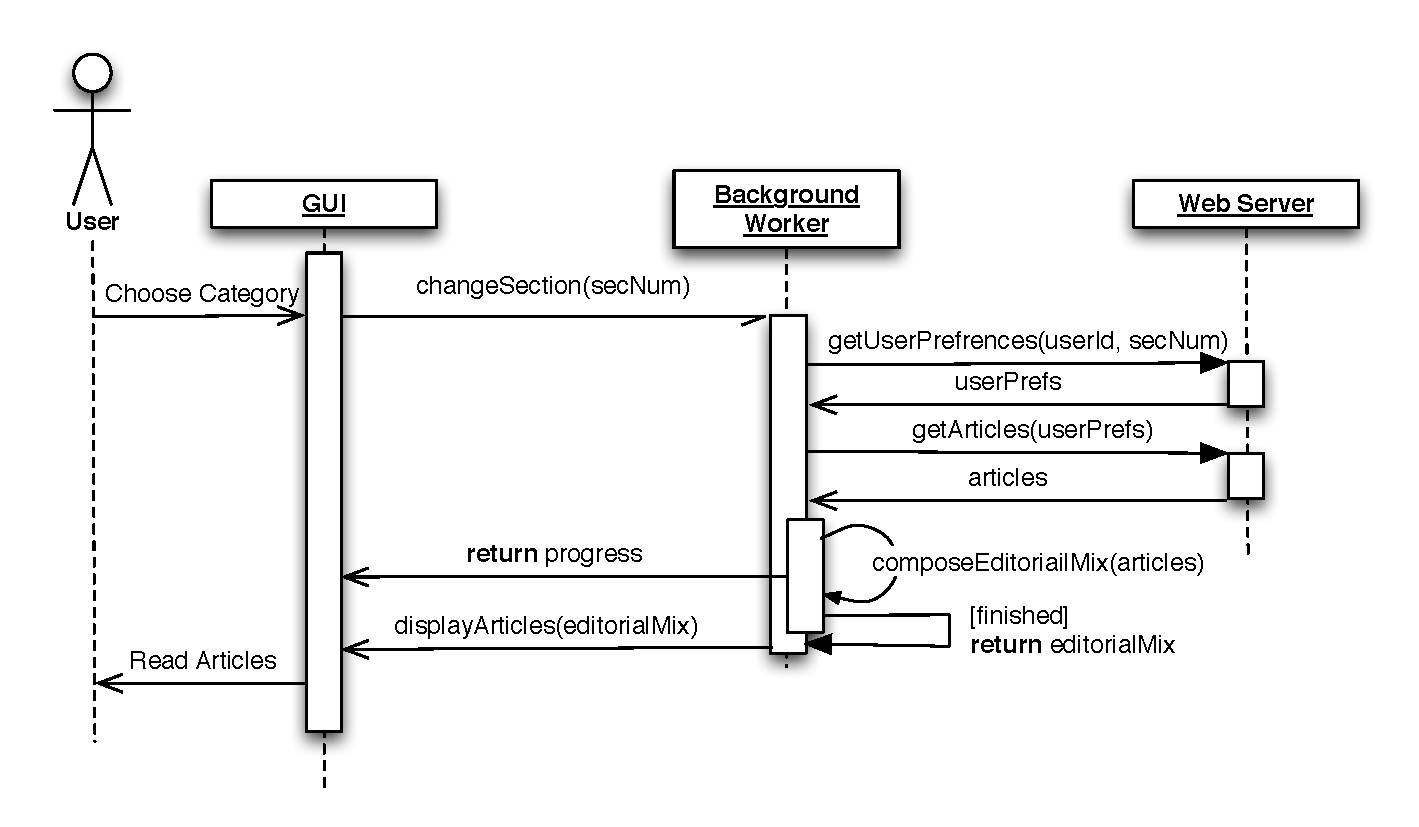
\includegraphics[width=.8\largefigure]{img/sequence}
%	}
%	\marginnote{
%	\vspace{-50pt}
%	\begin{minipage}{\marginparwidth}
%		\caption{A sequence diagram from when the user chooses a topic category until reading articles. \texttt{secNum} is a section number, (front page is section $0$), \texttt{userId} the user id, \texttt{%userPrefs} the user preferences on a given section and \texttt{articles} is a library of articles to compose the editorial mix of.}
%	\label{fig:sequence}
%		\end{minipage}
%	}
%\end{figure}
\begin{figure}[h!tp]
	\centering
	
	\def\mygraphic{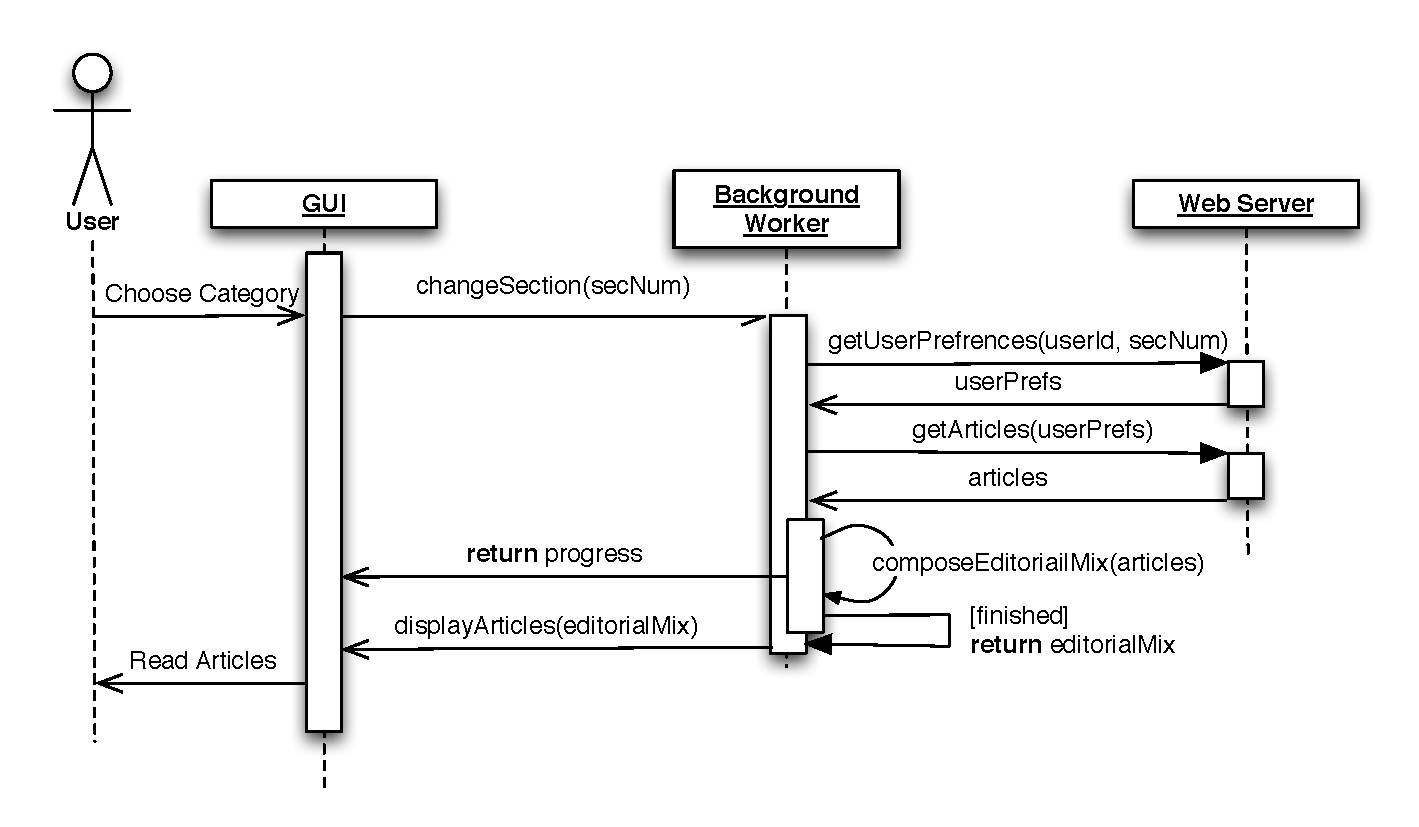
\includegraphics[width=\textwidth]{img/sequence}}
	%\newlength{\graphicheight}
	\settoheight\graphicheight{\mygraphic}
	\mygraphic
	\marginnote{
	\begin{minipage}{\marginparwidth}
		\vspace{-\graphicheight}%
		\caption{A sequence diagram from when the user chooses a topic category until reading articles. \texttt{secNum} is a section number, (front page is section $0$), \texttt{userId} the user id, \texttt{userPrefs} the user preferences on a given section and \texttt{articles} is a library of articles to compose the editorial mix of.}
		\label{fig:sequence}
		\vspace{\graphicheight}
		\end{minipage}
	}
\end{figure}
%\begin{figure}[h!tp]
%	\myfloatalign
%		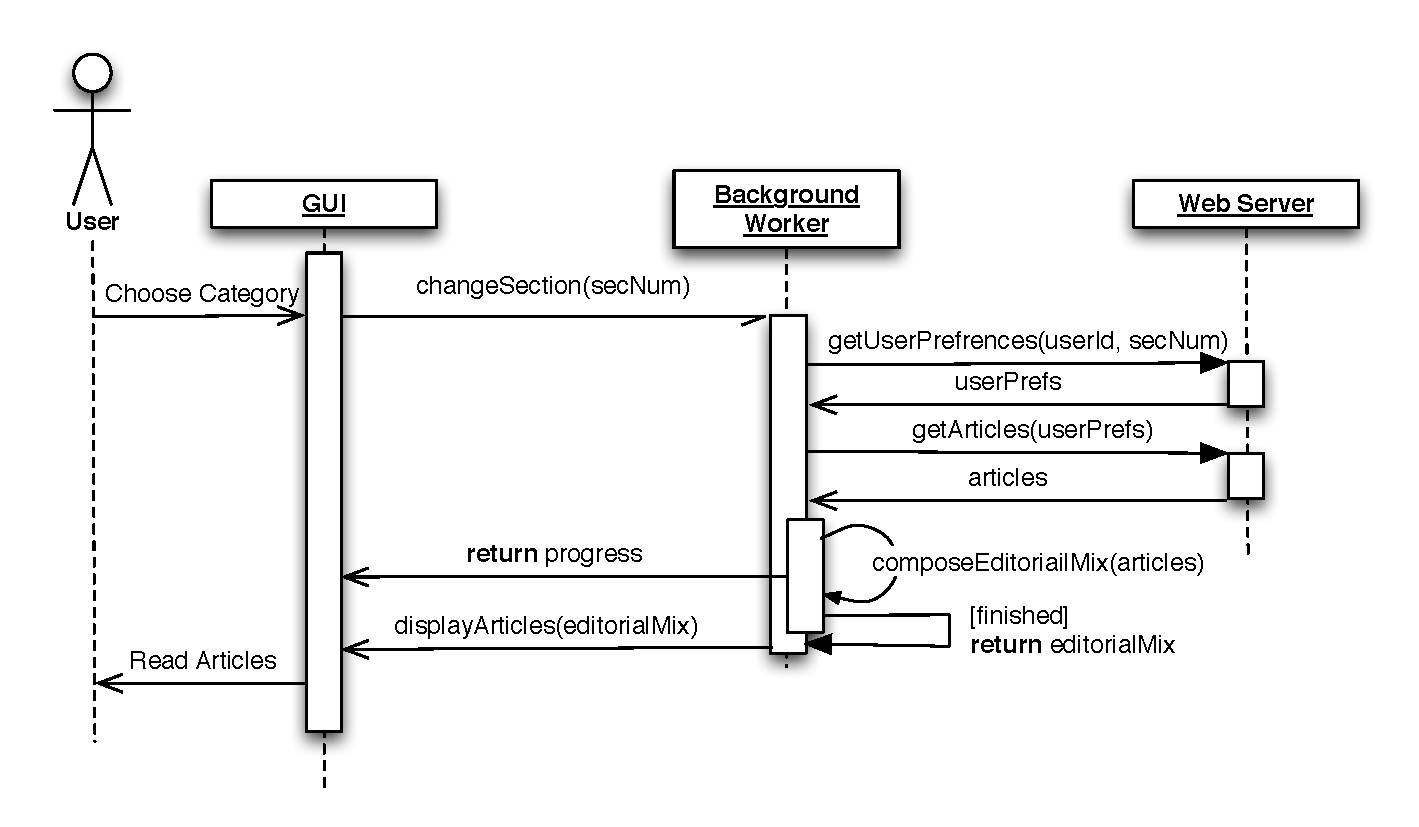
\includegraphics[width=\textwidth]{img/sequence}
%	\caption{The figure shows a sequence diagram from when the user chooses a topic category until he can read articles from this topic. \texttt{secNum} is the section number to display (the front page is section 0), \texttt{userId} is a string that identifies the user, \texttt{userPrefs} is the user preferences on the specific section and \texttt{articles} is the library of articles to compose the editorial mix of.}
%	\label{fig:sequence}
%\end{figure}

When the application is opened, or the application is changed to display a section, a background worker is initialised to compose its containing mix of articles. Of cause, if the mix of articles in a section, or the front page, have already been computed, it should not have to recompute it. The background worker needs to get both the user preferences of the chosen topic category and articles that potentially fit the user preferences. While the worker computes the editorial mix it sends messages to the user interface about the progress, to provide feedback to the user. When it finishes the user interface is asked to display the articles.



\subsection{Constraint Personalisation Library}

\subsubsection{Data Structure}
\subsubsection{General Purpose Solver}

\subsection{Backend worker.js}
  - Lazy Loading Sections
  - Knowledge Passing

worker i tråd for sig selv, men samme proces

worker.js to create a background worker to perform the constriant programming.

Model-View-Control using backbone.js

Paging: single page web apps + manipulation the browser history \url{https://developer.mozilla.org/en/DOM/Manipulating_the_browser_history}

Preference ordering of hard constraints or division between preference constraints and hard constraints.

Assignment from library in stead of arbitrary assignment? The latter is a more hypothetical approach. Providing the library as a constraint, where each variable assignment must have a unique combination from one of the possibilities of the constraint.
(sim,breaking,chars,date,sections?,columns):list
The former introduces an implicit constraint in that the general purpose solver can only choose from the library, thus can only choose a combination of values that exists.

Ranges can be optimised in space by converting them to integer ranges. This can be done by setting min = 0 and max = (b-a)/gap.

Furthermore each subdomain should be able to be represented by a set of ranges and atomic values. Propagating through values causes many iterations and a whole range may be discarded by looking at its maximum and minimum value. However, if the range holds a potential valid value (solution to a variable) it can be divided into smaller ranges and their minimum and maximum values may be examined. This divide-and-conquer technique may continue until the search reaches atomic values (determined by the gap value of the range). If some atomic values and ranges seems to fulfil the constraints they should be returned. And the subdomain now consists of both ranges and atomic values.

Optimal/promising
fixed budget computation

The library could take any combination of constraints and then organise them into conjunctions of disjunctions, with the constraints taking fewer values first.

In the implementation this is done by hand, so the program takes conjunctions of disjunctions of constraints organised with constraints that takes fewer values first. Constraint weighing could also help organising the disjunctions and furthermore lead the search to concentrate on variables that is bound by these constraints. (p. 222 AIRussel).

Constraints should point to specific variables, this makes it somewhat rigid/ineffective because I have to write at global constraint that accounts for everything (ineffective in propagation -- might also be a problem if it does not show progress in changing values, i.e.\ it is a hard constraints and not returning a cost of the set of values.) or divide it into smaller constraints separated by an `or' (v). The latter is ineffective because there would should be a combination of constraints accounting for every situation, e.g. if the first variable is satisfying an unary constraint, the next say 3 variables (if the problem holds 4 variables) could satisfy three unary constraints, an unary and a binary (two combinations exists) or a constraint that takes three variables. This grows fast with the number of constraints.

\todo[inline]{Does it make sense that a continuous range cannot have specific values removed? Should it be possible for it be divided into subranges if the user decides to remove a range of values in between its domain of [min;max]?}

Pool of workers to compute sections and send results to another worker to handle front page articles. Or, a lazy load approach where the front page is computed and then sections are computed with hard constraints that manages placement of articles within the given sections, e.g.\ if an article from the front page has the potential to be placed in only one section the constraint should state this, but it would demand cross-worker-constraints to handle if an article from the front page has the potential to be placed in more section (i.e.\ \texttt{xor}). color

Reducing constraints to binary constraints.

\todo[inline]{Implement visual difference between featured articles and non-featured articles.}

% section design (end)